\documentclass[tikz,border=6pt]{standalone}
\usepackage{amsmath,amssymb,mathtools}
\usepackage{xcolor}
\usepackage{tikz}
\usetikzlibrary{arrows.meta,calc,positioning,decorations.pathmorphing}

\definecolor{cobalt}{HTML}{2b4c7e}
\definecolor{navyhead}{HTML}{1a365d}
\definecolor{boxblue}{HTML}{eef3fa}
\definecolor{boxgreen}{HTML}{eaf6f0}
\definecolor{ruleblue}{HTML}{2b6cb0}
\definecolor{rulegold}{HTML}{b7791f}
\definecolor{rulered}{HTML}{c0392b}
\definecolor{rulegreen}{HTML}{1f8a5f}

\begin{document}
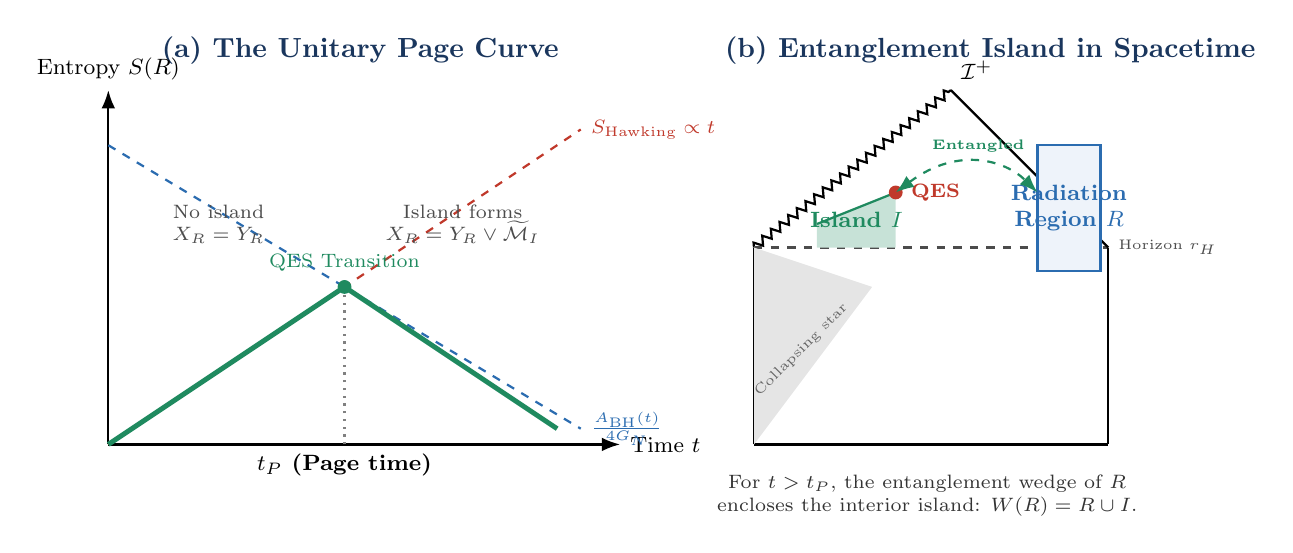
\begin{tikzpicture}[>=Latex, font=\small]

  % ================= PANEL A: THE PAGE CURVE =================
  \begin{scope}[shift={(0,0)}]
    \node[font=\bfseries\normalsize\color{navyhead}, align=center] at (3.2, 5.0) 
      {\textbf{(a)} The Unitary Page Curve};

    % Axes
    \draw[->, thick] (0, 0) -- (6.5, 0) node[right, font=\footnotesize] {Time $t$};
    \draw[->, thick] (0, 0) -- (0, 4.5) node[above, font=\footnotesize] {Entropy $S(R)$};

    % Curves
    % 1. Hawking's radiation calculation (rising monotonically)
    \draw[thick, dashed, color=rulered] (0, 0) -- (6.0, 4.0) 
      node[right, font=\scriptsize\color{rulered}] {$S_{\text{Hawking}} \propto t$};

    % 2. Bekenstein-Hawking Area of remaining black hole (decreasing)
    \draw[thick, dashed, color=ruleblue] (0, 3.8) -- (6.0, 0.2) 
      node[right, font=\scriptsize\color{ruleblue}] {$\frac{A_{\text{BH}}(t)}{4G_N}$};

    % 3. Page curve (Unitary result: minimum of the two)
    \draw[line width=1.8pt, color=rulegreen] (0, 0) -- (3.0, 2.0) -- (5.7, 0.2);

    % Page time marker
    \draw[dotted, thick, gray] (3.0, 0) -- (3.0, 2.0);
    \fill[rulegreen] (3.0, 2.0) circle (2.5pt);
    \node[below, font=\footnotesize\bfseries] at (3.0, 0) {$t_P$ (Page time)};
    \node[above=2pt, font=\scriptsize\color{rulegreen}, align=center] at (3.0, 2.0) 
      {QES Transition};

    % Annotations
    \node[font=\scriptsize\color{black!70}, align=center] at (1.4, 2.8) 
      {No island\\$X_R = Y_R$};
    \node[font=\scriptsize\color{black!70}, align=center] at (4.5, 2.8) 
      {Island forms\\$X_R = Y_R \vee \widetilde{\mathcal{M}}_I$};
  \end{scope}

  % ================= PANEL B: PENROSE DIAGRAM & ISLAND =================
  \begin{scope}[shift={(8.2,0)}]
    \node[font=\bfseries\normalsize\color{navyhead}, align=center] at (3.0, 5.0) 
      {\textbf{(b)} Entanglement Island in Spacetime};

    % Spacetime boundaries
    % Center r=0
    \draw[thick] (0, 0) -- (0, 2.5);
    % Future singularity (wavy line)
    \draw[decorate, decoration={zigzag, segment length=4pt, amplitude=1.5pt}, thick, color=black] 
      (0, 2.5) -- (2.5, 4.5);
    % Null horizon
    \draw[thick, dashed, color=black!70] (0, 2.5) -- (4.5, 2.5) node[right, font=\tiny] {Horizon $r_H$};
    % Future null infinity Scri+
    \draw[thick] (4.5, 2.5) -- (2.5, 4.5) node[above right, font=\footnotesize] {$\mathcal{I}^+$};
    % Past null infinity Scri-
    \draw[thick] (4.5, 0) -- (4.5, 2.5);
    % Past boundary
    \draw[thick] (0, 0) -- (4.5, 0);

    % Evaporation trajectory (matter collapsing)
    \fill[gray!20] (0,0) -- (1.5, 2.0) -- (0, 2.5) -- cycle;
    \node[font=\tiny\color{black!60}, rotate=45] at (0.6, 1.2) {Collapsing star};

    % Island region I (behind horizon)
    \fill[rulegreen!25] (0.8, 2.8) -- (1.8, 3.2) -- (1.8, 2.5) -- (0.8, 2.5) -- cycle;
    \draw[thick, rulegreen] (0.8, 2.8) -- (1.8, 3.2);
    \node[font=\footnotesize\bfseries\color{rulegreen}] at (1.3, 2.85) {Island $I$};

    % Quantum Extremal Surface (QES)
    \fill[rulered] (1.8, 3.2) circle (2.5pt) node[right=2pt, font=\scriptsize\bfseries\color{rulered}] {QES};

    % Radiation region R (far outside)
    \fill[boxblue, draw=ruleblue, thick] (3.6, 2.2) rectangle (4.4, 3.8);
    \node[font=\footnotesize\bfseries\color{ruleblue}, align=center] at (4.0, 3.0) {Radiation\\Region $R$};

    % Entanglement Wedge connection
    \draw[<->, dashed, thick, rulegreen] (1.8, 3.2) .. controls (2.6, 3.8) and (3.2, 3.6) .. (3.6, 3.2)
      node[midway, above, font=\tiny\bfseries, color=rulegreen] {Entangled};

    \node[below=2pt, font=\scriptsize\color{black!80}, align=center] at (2.2, -0.2) 
      {For $t > t_P$, the entanglement wedge of $R$\\encloses the interior island: $W(R) = R \cup I$.};
  \end{scope}

\end{tikzpicture}
\end{document}
